% Project:  Guomics-LaTex
% main.tex - main template
% content.tex - the body of course report 

\documentclass[11pt,a4paper]{article}
\usepackage[utf8]{inputenc}
\usepackage[
    top=1.7cm,
    bottom=1.7cm,
    left=1.7cm,
    right=1.7cm
]{geometry}
\usepackage{times}
\usepackage{microtype}
\usepackage{indentfirst}
\usepackage{array} % for customizing the table
\usepackage{float}
\usepackage{caption}
\usepackage{booktabs} % for better quality horizontal lines
\usepackage{amsmath}
\usepackage{amssymb}
\usepackage{xcolor}
\usepackage{graphicx}
\usepackage{listings}
\usepackage{algorithm}
\usepackage{algpseudocode}
\usepackage{hyperref}
\usepackage{float}
\usepackage[style=nature]{biblatex}
\usepackage[absolute,overlay]{textpos}
\usepackage{fancyhdr}
\usepackage{lastpage}
\usepackage{fancytabs}
\usepackage[parfill]{parskip}
\captionsetup[figure]{labelfont=bf}
\captionsetup[table]{labelfont=bf}



% ------------------------------------
% define new commands
\renewcommand{\figurename}{Fig.}
\renewcommand{\ttdefault}{cmtt}
\newcommand{\HRule}[1]{\rule{\linewidth}{#1}}
\newcommand{\name}{XXX XXX}
\newcommand{\ID}{xxxxxx}
\newcommand{\school}{Westlake University}
% ------------------------------------


\hypersetup{ % play with the different link colors here
    colorlinks,
    citecolor=blue,
    filecolor=blue,
    linkcolor=blue,
    urlcolor=blue
}
\definecolor{codegreen}{rgb}{0,0.6,0}
\definecolor{codegray}{rgb}{0.5,0.5,0.5}
\definecolor{codepurple}{rgb}{0.58,0,0.82}
\definecolor{backcolour}{rgb}{0.98,0.98,0.98}
\lstdefinestyle{mystyle}{
    backgroundcolor=\color{backcolour}, % background color
    commentstyle=\color{codegreen},     % comment style
    keywordstyle=\color{magenta},       % keyword style
    numberstyle=\tiny\color{codegray},  % number style
    stringstyle=\color{codepurple},     % string literal style
    basicstyle=\ttfamily\footnotesize,  % font style
    breakatwhitespace=false,            % automatic breaks only at whitespace
    breaklines=true,                    % automatic line breaking only at whitespace
    captionpos=b,                       % caption-position is bottom
    keepspaces=true,                    % keeps spaces in text
    numbers=none,                       % where to put the line-numbers
    numbersep=5pt,                      % how far the line-numbers are from the code
    showspaces=false,                   % show spaces adding particular underscores
    showstringspaces=false,             % underline spaces within strings
    showtabs=false,                     % show tabs within strings adding particular underscores
    tabsize=2,                          % sets default tabsize to 2 spaces
    frame=single,                       % adds a frame around the code
    rulecolor=\color{codegray},         
    framerule=0pt,                      % frame thickness
    abovecaptionskip=1em,
    belowcaptionskip=1em
}
\lstset{style=mystyle}
\setcounter{secnumdepth}{3}
\addbibresource{references.bib}

\pagestyle{fancy}
\fancyhf{} 
\fancyfoot[C]{\thepage} 
\renewcommand{\headrulewidth}{0pt} 
\renewcommand{\footrulewidth}{0pt} 
\setcounter{page}{1}


% ------------------------------------
% titlepage
\begin{document}
\begin{titlepage}
    \thispagestyle{fancy}
    \fancyfoot[C]{\thepage}
    % logo
    \centering
    \begin{textblock*}{5cm}(0.5cm, 1.1cm) 
        \noindent 
        
\includegraphics[width=0.6\linewidth]{figures/logo.png} 
    \end{textblock*} 
    \begin{textblock*}{5cm}(4cm, 1.2cm) 
        \noindent 
        
\includegraphics[width=0.7\linewidth]{figures/westlakelab.png}
    \end{textblock*}
    \begin{textblock*}{5cm}(6.5cm, 1.2cm) 
        \noindent
        
\includegraphics[width=0.28\linewidth]{figures/guomics.png}
    \end{textblock*}
    \begin{textblock*}{5cm}(9cm, 1.3cm) 
        \noindent
        \includegraphics[width=0.6\linewidth]{figures/WeCIP.png}
    \end{textblock*}
    \vspace*{10pt} 
    \HRule{1pt} 
    \begin{center}
    \parbox{\linewidth}{\centering\Huge\textbf{This is the title}}
    \end{center}
    \HRule{2pt}
    \vspace{2pt}
    
    \begin{center}
    \large
    \begin{minipage}[t]{0.3\textwidth}
    \centering
    \textbf{First Author}\textsuperscript{1,2,*}\thanks{These authors contributed equally to this work.} \\
    \texttt{iauthor@gmail.com}
    \end{minipage}
    \begin{minipage}[t]{0.3\textwidth}
    \centering
    \textbf{Second Author}\textsuperscript{2,3} \\
    \texttt{iiauthor@gmail.com}
    \end{minipage}
    \begin{minipage}[t]{0.3\textwidth}
    \centering
    \textbf{Third Author}\textsuperscript{1,2} \\
    \texttt{iiiauthor@gmail.com}
    \end{minipage} \\[1cm]
    \footnotesize
    \textsuperscript{1}Department Name, University Name ;
    \textsuperscript{2}Another Department, University Name ;
    \textsuperscript{3}Third Department, University Name ;
    \textsuperscript{*}Corresponding author
    \end{center}
    \vspace{1cm}


    
    \begin{minipage}{0.9\textwidth}
    \begin{center}
    \textbf{\large Abstract}
    \end{center}
    \large
    This study investigates the proteomic changes in Alzheimer disease associated with progressive amyloid-beta plaque and tau tangle pathologies. Through comprehensive proteomic analysis, we identified key protein alterations that correlate with disease progression. Our findings reveal significant changes in synaptic proteins, inflammatory markers, and metabolic enzymes. These results provide new insights into the molecular mechanisms underlying Alzheimer disease pathogenesis and suggest potential therapeutic targets for disease intervention.
    \end{minipage}


    \vspace{11cm}
    \begin{minipage}{0.9\textwidth}
    \begin{center}
    \end{center}
    \large
    \textbf{Keywords:} proteomics; mass spectrometry
    \end{minipage}
    

\end{titlepage}
% ------------------------------------


% ------------------------------------
% main body
\newpage
% main content
\pagestyle{fancy}
\fancyhf{}
\fancyhead[L]{
\begin{textblock*}{4cm}(0.5cm, 0.5cm) 
    \noindent 
    
\includegraphics[width=0.4\linewidth]{figures/logo.png} 
\end{textblock*} 
}
\fancyhead[C]{
\begin{textblock*}{4cm}(1.2cm, 0.55cm) 
    \noindent 
    
\includegraphics[width=0.5\linewidth]{figures/westlakelab.png}
\end{textblock*}
\begin{textblock*}{4cm}(2.7cm, 0.55cm) 
    \noindent
    
\includegraphics[width=0.2\linewidth]{figures/guomics.png}
\end{textblock*}
}
\fancyhead[R]{
\begin{textblock*}{4cm}(3cm, 0.6cm) 
    \noindent
    \includegraphics[width=0.4\linewidth]{figures/WeCIP.png}
\end{textblock*}
}
\fancyfoot[C]{\thepage}
\renewcommand{\headrulewidth}{0pt}
\renewcommand{\footrulewidth}{0pt}

\setcounter{page}{2}
\section{Introduction}
This document serves as a template for writing reports using \LaTeX. It includes sections for introduction, results, discussion, and methods, along with examples of how to use various \LaTeX\ features such as equations, tables, algorithms, and graphics.

This is paragragh 2. And this is paragraph 3. The spacing between these two paragraphs is set to 8pt, which can be adjusted as needed.

\section{Results}
\subsection{Results1}
This section summarizes the key findings of the  project. It highlights the main results and their implications for the field of study.
\subsection{Results2}
\section{Discussion}
The discussion section interprets the results in the context of existing literature. It explores the implications of the findings, potential limitations, and future directions for research.
\section{Conclusion}
This section summarizes the main findings of the report and their significance. It also suggests potential applications and future research directions.
\section{Materials and Methods}
This section describes the materials and methods used in the study. It provides detailed information on the experimental design, data collection, and analysis techniques employed in the research.
\subsection{Materials}
This section lists the materials used in the study, including any specific reagents, equipment, or software that were essential for conducting the research.
\subsection{Methods}
This section outlines the methods used in the study, including experimental protocols, data analysis techniques, and any statistical methods applied to interpret the results. It provides enough detail for others to replicate the study if desired.
\section{Data Availability}
This section describes the availability of the data used in the study. It includes information on how to access the data, any restrictions on its use, and any relevant repositories or databases where the data can be found.
\section{Code Availability}
This section provides information on the availability of the code used in the study. It includes links to repositories or platforms where the code can be accessed, as well as any instructions for running or modifying the code.
\section{Acknowledgements}
This section acknowledges individuals, organizations, or funding sources that contributed to the study but did not meet the criteria for authorship. It may include funding agencies, collaborators, or institutions that provided support.
\section{Author Contributions}
This section outlines the contributions of each author to the study. It specifies who was responsible for conceptualization, methodology, data collection, analysis, writing, and any other relevant tasks. This helps clarify the roles of each author in the research process.
\section{Competing Interests}
This section declares any potential conflicts of interest that may have influenced the study. It includes financial interests, personal relationships, or other affiliations that could be perceived as influencing the research outcomes.
\printbibliography[title={References}]
\newpage
% ------------------------------------
\begin{figure}[htbp]
    \begin{center}
        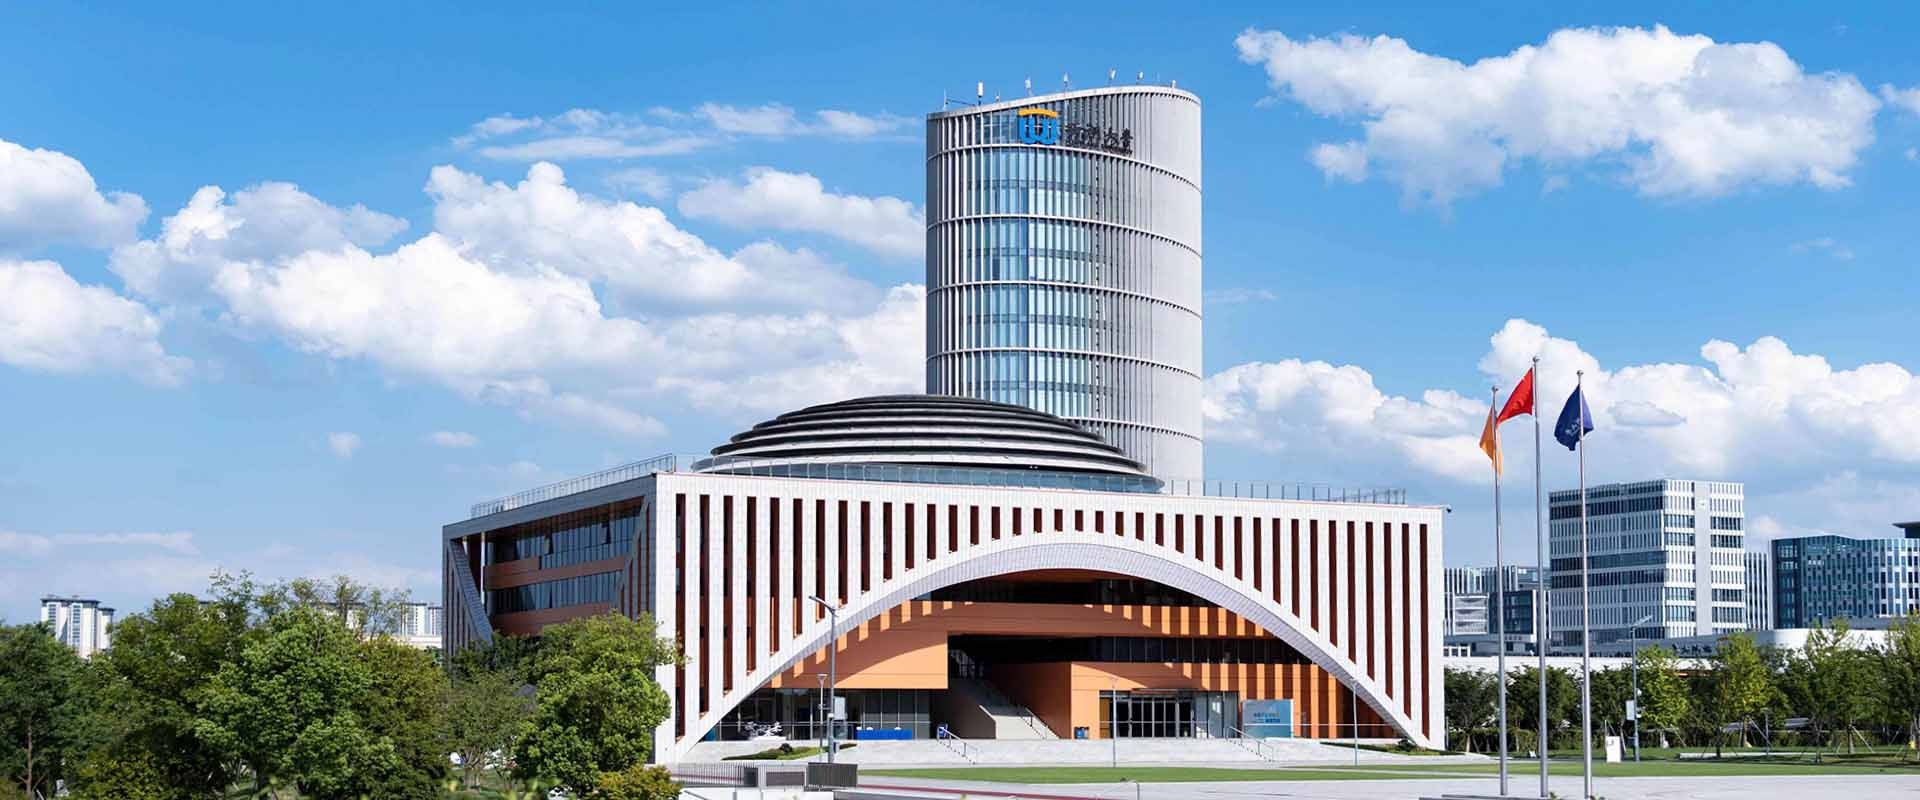
\includegraphics[width=0.8\textwidth]{./figures/westlake.jpg}
    \end{center}
            \caption{This photo was taken by Kairos at Westlake University. (A) A beautiful view of Westlake University. (B) A photo of the Westlake University library.}
    \label{fig1}
\end{figure}

\newpage




\section*{\LaTeX Templates} 
\subsection*{Basic Commands}
\LaTeX\ is a powerful typesetting system that is widely used for academic and scientific documents. Below are some of the fundamental commands you'll use frequently (All used in \textcolor{blue}{content.tex}).

Commands: 
\begin{table}[h]
    \centering
    \begin{tabular}{lll}
        \textcolor{red}{\textbackslash section}         & \textcolor{red}{\textbackslash subsection}      & \textcolor{red}{\textbackslash subsubsection}   \\
        \textcolor{red}{\textbackslash centering}       & \textcolor{red}{\textbackslash flushleft}       & \textcolor{red}{\textbackslash flushright}      \\
        \textcolor{red}{\textbackslash caption}         & \textcolor{red}{\textbackslash includegraphics} & \textcolor{red}{\textbackslash label}           \\
        \textcolor{red}{\textbackslash cite}            & \textcolor{red}{\textbackslash ref}             & \textcolor{red}{\textbackslash url}             \\
    \end{tabular}
\end{table}

Environments:
\begin{table}[h]
    \centering
    \begin{tabular}{lll}
        \textcolor{blue}{\textbackslash equation}    & \textcolor{blue}{\textbackslash table}       & \textcolor{blue}{\textbackslash lstlisting}  \\
        \textcolor{blue}{\textbackslash algorithm}   & \textcolor{blue}{\textbackslash figure}      & \textcolor{blue}{\textbackslash align*}      \\
    \end{tabular}
\end{table}

\subsection*{Working with Maths}
\LaTeX\ makes your math formulas look clean and professional, which is why I love it so much. We could use two writing modes, \textit{inline} and \textit{display} math mode.

Let's start with inline math mode. You can use dollar signs \texttt{\$...\$} to enclose a mathematical expression. For example, typing \texttt{\$E=mc\^{}2\$} will display as $E=mc^2$. And if we would like to make sure equations could be numbered or unnumbred, such as 

\begin{equation}
    p^{*}(y_{w}\succ y_{l} \mid x) = \frac{\exp(r^{*}(x,y_{w}))}{\exp(r^{*}(x,y_{w}))+\exp(r^{*}(x,y_{l}))}. \label{eq1}
\end{equation}

\begin{align*}
    p^{*}(y_{w}\succ y_{l} \mid x) = \frac{\exp(r^{*}(x,y_{w}))}{\exp(r^{*}(x,y_{w}))+\exp(r^{*}(x,y_{l}))}. 
\end{align*}

The corresponding code is:
\begin{lstlisting}[language=TeX]
\begin{equation}
    p^{*}(y_{w}\succ y_{l} \mid x) = \frac{\exp(r^{*}(x,y_{w}))}{\exp(r^{*}(x,y_{w}))+\exp(r^{*}(x,y_{l}))}. \label{eq1}
\end{equation}

\begin{align*}
    p^{*}(y_{w}\succ y_{l} \mid x) = \frac{\exp(r^{*}(x,y_{w}))}{\exp(r^{*}(x,y_{w}))+\exp(r^{*}(x,y_{l}))}. 
\end{align*}
\end{lstlisting}

Moreover, when you need to align multiple equations, please use the \textit{align} environment. Even you could mix \textit{align} and \textit{equation} environments. Here, I strongly recommend this website \url{https://www.latexlive.com}, which is an online formula editor that allows you to create and edit \LaTeX\ equations directly in your browser.


\subsection*{Tables}
TablesGenerator \url{https://www.tablesgenerator.com/} is a useful online tool for creating \LaTeX\ tables. It allows you to design, export, and embed tables without needing to install any software. Sometimes manually typing out tables could be pretty troublesome, but using this website makes it more convenient.

\begin{table}[h!]
\centering
\begin{tabular}{|l|l|l|}
\hline
a & b & c \\ \hline
d & e & f \\ \hline
\end{tabular}
\caption{Table example}
\label{tab1}
\end{table}

\subsection*{Code and Algorithm}
The \textit{listings} package offers syntax highlighting, line numbering, and other features that make the code more readable. Here’s a simple example of a Python function:

\begin{lstlisting}[language=Python]
def hello_world():
    print("Hello, world!")  # code comment
\end{lstlisting}

For presenting algorithms, \LaTeX\ offers the \textit{algorithm} and \textit{algorithmic} environments, which allow you to structure and annotate algorithms clearly. The following example demonstrates the Generative Adversarial Imitation Learning (GAIL) algorithm, a method used in reinforcement learning:

\begin{algorithm}
    \caption{Generative Adversarial Imitation Learning (GAIL)}
    \label{alg1}
    \begin{algorithmic}[1]
    \State Input: Expert trajectories $\tau_E \sim \pi_E$, initial policy and discriminator parameters $\theta_0, w_0$
    \For{$i=0,1,2, \ldots$}
        \State Sample trajectories $\tau_i \sim \pi_{\theta_i}$
        \State Update the discriminator parameters from $w_i$ to $w_{i+1}$ with the gradient
        $$
            \hat{\mathbb{E}}_{\tau_i}\left[\nabla_w \log \left(D_w(s, a)\right)\right]+\hat{\mathbb{E}}_{\tau_E}\left[\nabla_w \log \left(1-D_w(s, a)\right)\right]
        $$
        \State Take a policy step from $\theta_i$ to $\theta_{i+1}$, using the TRPO rule with cost function $\log \left(D_{w_{i+1}}(s, a)\right)$. Specifically, take a KL-constrained natural gradient step with
        \begin{align*}
            & \hat{\mathbb{E}}_{\tau_i}\left[\nabla_\theta \log \pi_\theta(a \mid s) Q(s, a)\right]-\lambda \nabla_\theta H\left(\pi_\theta\right), \\
            & \text { where } Q(\bar{s}, \bar{a})=\hat{\mathbb{E}}_{\tau_i}\left[\log \left(D_{w_{i+1}}(s, a)\right) \mid s_0=\bar{s}, a_0=\bar{a}\right]
        \end{align*}
    \EndFor
    \end{algorithmic}
\end{algorithm}


\subsection*{Graphics}
To include graphics in our \LaTeX\ document, we could use \textit{figure} environment along with \textit{graphicx} package. Below is an example of how to insert an image:

\begin{lstlisting}[language=TeX]
\begin{figure}[htbp]
    \begin{center}
        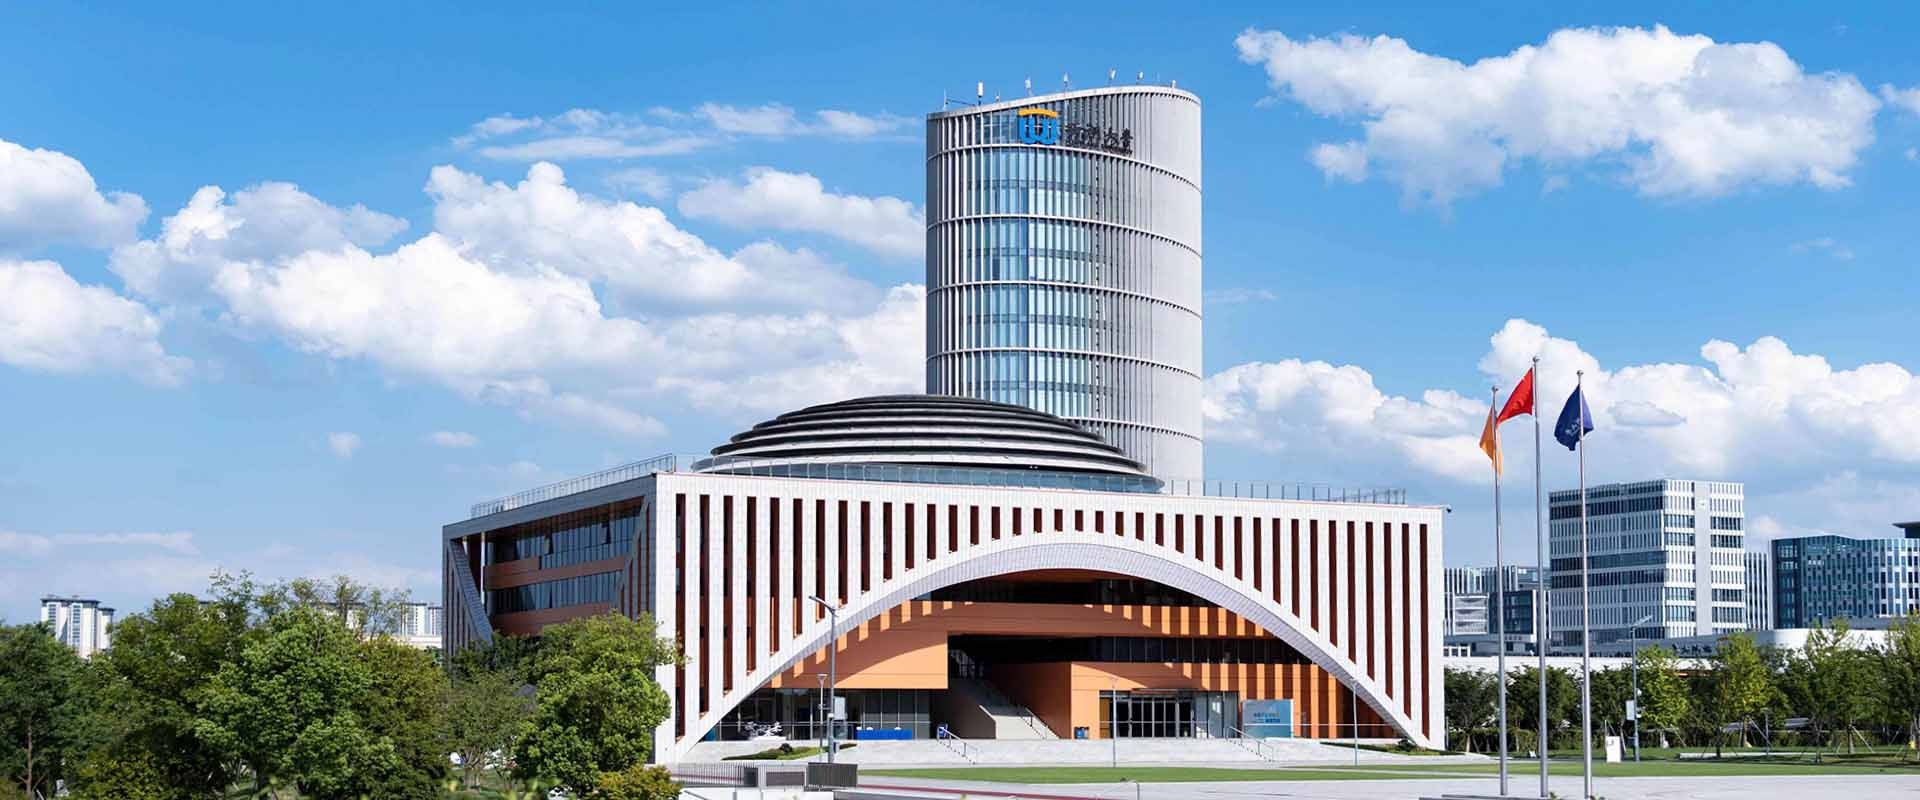
\includegraphics[width=0.8\textwidth]{./figures/westlake.jpg}
    \end{center}
            \caption{This photo was taken by Kairos at Westlake University.}
    \label{fig1}
\end{figure}
\end{lstlisting}



\subsection*{Referencing and Hyperlinking}
\subsubsection*{Linking}
To create references and hyperlinks, we could use the hyperref package.
\LaTeX\ allows us to link to figures (Fig. \ref{fig1}), tables (Table \ref{tab1}), equations (Eq. \ref{eq1}), algorithms (Algorithm \ref{alg1}), and external URLs.

\subsubsection*{Bibliography}
To cite references, please use \textbackslash \texttt{cite} command followed by the citation key from .bib file. We could include those keys in .bib file to manage references for articles \cite{Article2024}, books \cite{Book2024}, websites \cite{Website2024}, and conference papers \cite{Inproceeding2024}. Here are some styles:

\begin{lstlisting}
@article{Article2024,
  author  = {Author},
  title   = {Sample Article Title},
  journal = {Journal of Samples},
  year    = {2024},
  volume  = {10},
  number  = {2},
  pages   = {123-145}
}

@book{Book2024,
  author    = {Author},
  title     = {Sample Book Title},
  publisher = {Publisher Name},
  year      = {2024},
  address   = {Publisher Address},
  edition   = {2nd}
}

@online{Website2024,
  author  = {Author},
  title   = {Sample Webpage Title},
  year    = {2021},
  url     = {http://www.example.com},
  urldate = {2024-07-22}
}

@inproceedings{Inproceeding2024,
  author       = {Author},
  title        = {Sample Conference Paper Title},
  booktitle    = {Proceedings of the Sample Conference},
  year         = {2024},
  editor       = {Editor Name},
  volume       = {1},
  series       = {Series Name},
  pages        = {45-60},
  address      = {Conference Address},
  month        = {7},
  organization = {Conference Organization}
}
\end{lstlisting}


% ------------------------------------







% ------------------------------------


\end{document}